\section{Basic Propagation Models}
\label{sec:propmodels}
\begin{aautop}
    This section will describe some simple propagation models and terms that can be used to establish the maximum obtainable communication range given the maximum path loss computed in a link budget. 
\end{aautop}

The simplest propagation model is the free-space path loss, which is given in Equation~\ref{eq:fspl}.
The free-space path loss is, however, rarely appropriate, since it does not take trees, buildings, etc.\ into account \cite{balanis2012antenna}. There are, however, a myriad of empirical models which are based on actual measurements. The drawback is that these empirical models tend not to be general and a given model might not be suited for two different cities. This results in that empirical models often are grouped into three main branches: Foliage, terrain, and city models \cite{goldsmith2005wireless}. For foliage areas models such as the Weissbergers model and the ITU Vegetation model can be used \cite{goldsmith2005wireless}. For terrain areas, models such as the Egli or Longley-Rice model are used \cite{goldsmith2005wireless}. To model the path loss in cities, the Young, Okumura, Hata, or the COST 231 models can be used \cite{goldsmith2005wireless}. It should be noted that some of these models are not usable in upper LTE frequency range, and thus care should be taken when applying these models. 

\subsection{Multipath}
The multipath effect exists when a wave and/or multiple waves are scattered, such that the receiver experiences multiple copies of the same wave coming from different directions. In areas where there is no ground or other obstacles (free-space) the multipath effect does not exist. The simplest multipath case is the two-ray case, where the surface of the earth is included, in this case there will be a single reflection from the earth and thus multiple paths from the transmitter to the receiver \cite{parsons2000mobile}. This scenario is illustrated in Figure~\ref{fig:mul_tworay}.

\begin{figure}[htbp]
    \centering
    \begin{subfigure}[b]{0.6\textwidth} 
        \centering
        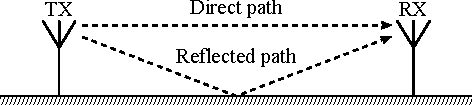
\includegraphics[scale=0.8]{img/analysis/tworay}
        \caption{Two ray path model.}
        \label{fig:mul_tworay}
    \end{subfigure}
    \\
    \begin{subfigure}[b]{0.7\textwidth} 
        \centering
        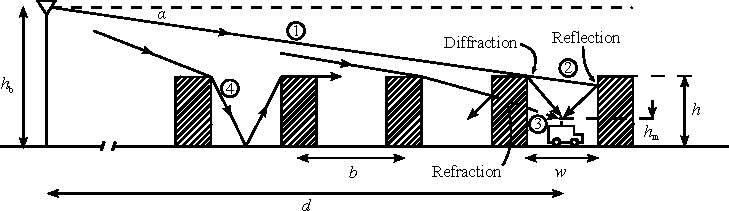
\includegraphics{img/analysis/parsons_multipath}
        \caption{Reflection and diffraction causing the multi-path effect \cite{parsons2000mobile}. The signal received by the car consists of diffracted, reflected, and refracted waves but no direct line-of-sight component.}
        \label{fig:mul_reflec_diffrac}
    \end{subfigure}
    \caption{Two ray model and different multipath effects.}
\end{figure}

The multipath effect will be greatest in urban environments, where several buildings and other obstacles are present. If the surface is rough, scattering will also take place. This is the phenomenon where a single incoming wave scatters into multiple reflections. In addition to this there is also diffraction where a wave front is ``bend'' at the edges of buildings, which is illustrated in Figure~\ref{fig:mul_reflec_diffrac}. Multipath results in a negative effect on the throughput. However, with MIMO, the multipath effects are now exploited positively to increase throughput and channel stabilization \cite{parsons2000mobile}.

\subsection{Fading}
The signal strength in a wireless channel is constantly fluctuating. These variations are represented by fading. The variations can be caused by scattering, reflections, blockage etc. Based on the type of variation, the fading is grouped in \emph{small scale fading} and \emph{large scale fading}. Large scale fading is typically caused by large objects, such as hills and buildings, where small scale fading occurs over small travel distances due to constructive or destructive adding of the multipath waves \cite{parsons2000mobile}.

By superimposing the path loss with small scale fading and large scale fading, the combined model, which represents the total propagation and path loss, is obtained. This is illustrated in Figure~\ref{fig:mul_combined}. 

\begin{figure}[htbp]
    \centering
    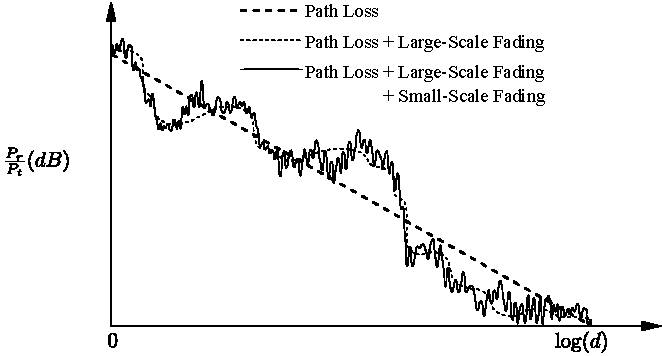
\includegraphics{img/analysis/goldsmith_combined}
    \caption{Combined path loss model with large- and small-scale fading \cite{goldsmith2005wireless}.}
    \label{fig:mul_combined}
\end{figure}

\subsection{Empirical Models}
This section will describe some of the city-models that are often used in estimating the path loss. 

\subsubsection{Hata Model}
The Hata model is a mathematical model derived from the graphical Okumura model, which is based on measurements from Tokyo in 1960 in the frequency range \SIrange{200}{1920}{MHz}. The model is divided into three groups: Urban, suburban, and open areas which are defined in dB in Equation~\ref{eqn:hataModelUrban}, Equation~\ref{eqn:hataModelSubUrban}, and Equation~\ref{eqn:hataModelOpen}, respectively \cite{Seybold2005introduction}.
\begin{align} %%
    \label{eqn:hataModelUrban}
    L_{50} = L_{50}(\text{urban}) = 69.55+26.12 \log(f_c) - 13.82 \log(h_t) -a(h_r) + [44.9-6.55 \log(h_t)] \log(d)
\end{align} 
where
\begin{where}
\item [$f_{c}$] Center frequency in \si{MHz} and in the range: $150 < f_c < 1500$.
\item [$h_t$] Height in meters, which must satisfy $30 < h_t < 200$.
\item [$d$] Distance in km which must satisfy $1 < d < 20$.
\item [$a(h_r)$] The mobile antenna height correction factor. Defined in Equation~\ref{eqn:hataModelahrSmall} \cite{Seybold2005introduction} for small and medium sized cities. Defined in Equation~\ref{eqn:hataModelahrLarge} \cite{Seybold2005introduction} for a large city. 
\end{where}
\begin{align} %%
\label{eqn:hataModelahrSmall}
a(h_r) &= (1.1 \log(f_c)-0.7]h_r - [1.56 \log(f_c)-0.8)\quad\text{if } \SI{1}{m} \leq h_r \leq \SI{10}{m} \\
\label{eqn:hataModelahrLarge}
a(h_r) &= 
  \begin{cases}
    8.29(\log(1.54 h_r))^2 -1.1 & \text{ if } f_c \leq \SI{200}{MHz}, \\
    3.2(\log(11.75 h_r))^2 -4.97 & \text{ if } f_c \leq \SI{400}{MHz} 
  \end{cases}\\
\label{eqn:hataModelSubUrban}
L_{50}(dB) &= L_{50}(\text{urban})-4.78(\log(f_c))^2 + 18.33 \log(f_c) - 40.94 \\
\label{eqn:hataModelOpen}
L_{50}(dB) &= L_{50}(\text{urban})-2 \left(\log\left( \frac{f_c}{28} \right) \right)^2 -5.4 
\end{align} 
This extension to the Okumura model is often used in practical applications since it is easier to apply than the Okumura model. However, it only handles frequencies up to \SI{1500}{MHz}, which lead to the COST 231 model being developed.

\subsubsection{COST 231 Model}
%COST 231 Model
The COST 231 model is an extension of the Hata model. It includes the PCS bands \SIrange{1800}{1900}{MHz} which makes it an ideal model for many wireless personal communication systems (GSM etc.). The path loss is given by Equation~\ref{eqn:COSTModel} in dB \cite{Seybold2005introduction} and the model is valid in the frequency range of  \SIrange{1500}{2000}{MHz}, link distance from \SI{1}{km} to \SI{20}{km}, a transmitter antenna height of \SIrange{30}{200}{m}, and a receiver height of \SIrange{1}{10}{m} \cite{Seybold2005introduction}. It should also be stated that the model is restricted to applications where the base station antenna is above adjacent roof tops \cite{itu2002report}.
\begin{align} 
    \label{eqn:COSTModel} %%
    L_{50}(dB) = 46.3+33.9 \log(f_c)-13.82 \log(h_t)-a(h_r)+[44.9-6.55 \log(h_t)] \log(d) + C 
\end{align} 
where 
\begin{where}
\item [$f_c$] Frequency in \si{MHz}.
\item [$h_t$] Transmitter height in \si{m}. 
\item [$h_r$] Receiver height in \si{m}.
\item [$a(h_r)$] Mobile antenna height correction factor from Equation~\ref{eqn:hataModelahrSmall} and Equation~\ref{eqn:hataModelahrLarge}.
\item [$d$] Distance of propagation.
\item [$C$] \SI{0}{dB} for suburban and medium cities with medium tree density, 3 dB for metropolitan centers. 
\end{where}

\subsubsection{Extended COST}
%Extended COST 
An extension to the COST 231 model is described in a ITU (International Telecommunication Union) report \cite{itu2002report} and this model extends the COST 231 such that it is accurate up to \SI{3}{GHz}. The path loss model for an urban environment in the range of \SIrange{2000}{3000}{MHz} is given by \cite{itu2002report}
\begin{equation}%% 
\label{eqn:COSTModelExtended}
\begin{aligned}
    L &= 46.3 + 33.9 \log(2000) + 10 \log\left(\frac{f_c}{2000}\right) \\
        &- 13.82 \log(\text{max}\{30,h_t\}) + [44.9 -6.55 \log(\text{max}\{30,h_t\})] (\log(d))^{\alpha} - a(h_r) - b(h_t)
%L = 46.3 + 33.9\log(2000) + 10\log(\frac{f_c}{2000}) − 13.82\log(max{30,H_t}) +[44.9 − 6.55\log(max{30,H_t})](\log(d))\alpha −a(H_r)−b(H_t)
\end{aligned}
\end{equation} 
where
\begin{where}
\item [$f_c$] The frequency in \si{MHz}.
\item [$h_t$] Transmitter height in \si{m}. 
\item [$h_r$] Receiver height in \si{m}.
\item [$a(h_r)$] The mobile antenna height correction factor given in Equation~\ref{eqn:COSTModelExtendedhr}.
\item [$b(h_t)$] Transmitter height correction factor given in Equation~\ref{eqn:COSTModelExtendedht}.
\item [$\alpha$] Given in Equation~\ref{eqn:aplhacostextended}.
\end{where}
\begin{align} %%
\label{eqn:COSTModelExtendedhr}
a(h_r)&=(1.1\log(f)-0.7) \min\{10,h_r\}-(1.56\log(f)-0.8)+\max\left\{0,20\log\left(\frac{h_r}{10}\right)\right\}\\
\label{eqn:COSTModelExtendedht}
b(h_t)&= \min\left\{0,20\log\left(\frac{h_t}{30}\right)\right\}\\
\label{eqn:aplhacostextended}
\alpha &= 
  \begin{cases}
      1 & \text{ if } (d \leq \SI{20}{km}) \\
    1+(0.14+\num{1.87e-4} f + \num{1.07e-3} h_t & \text{ if } (\SI{20}{km} < d \leq \SI{100}{km})
  \end{cases}
\end{align} 

\begin{aautail}
    In this section, basic propagation models were described, making it possible to predict the communication distance given a certain maximum path loss. In the next section, the effect of having a user present in a mobile communication system will be described.
\end{aautail}
